%This is chapter 3
%%=========================================
\chapter{Design and implementation of dragn}\label{prototype}
The architecture of the \textbf{dragn} (\textbf{D}istant \textbf{R}eading \textbf{A}nd \textbf{G}raph \textbf{N}odes) system and its design will be outlined in this chapter. Furthermore, each of the pipeline steps of the system will be detailed and the algorithms and calculations performed therein explained. Each of the steps produces output that is written to the disk and persists even after that part of the system finishes for further analysis and use in other research.\\
The emphasis of this chapter is not only on the internal part of the system, the back end, but the interface or front end as well.\\
\begin{figure}[H]
    \centering
    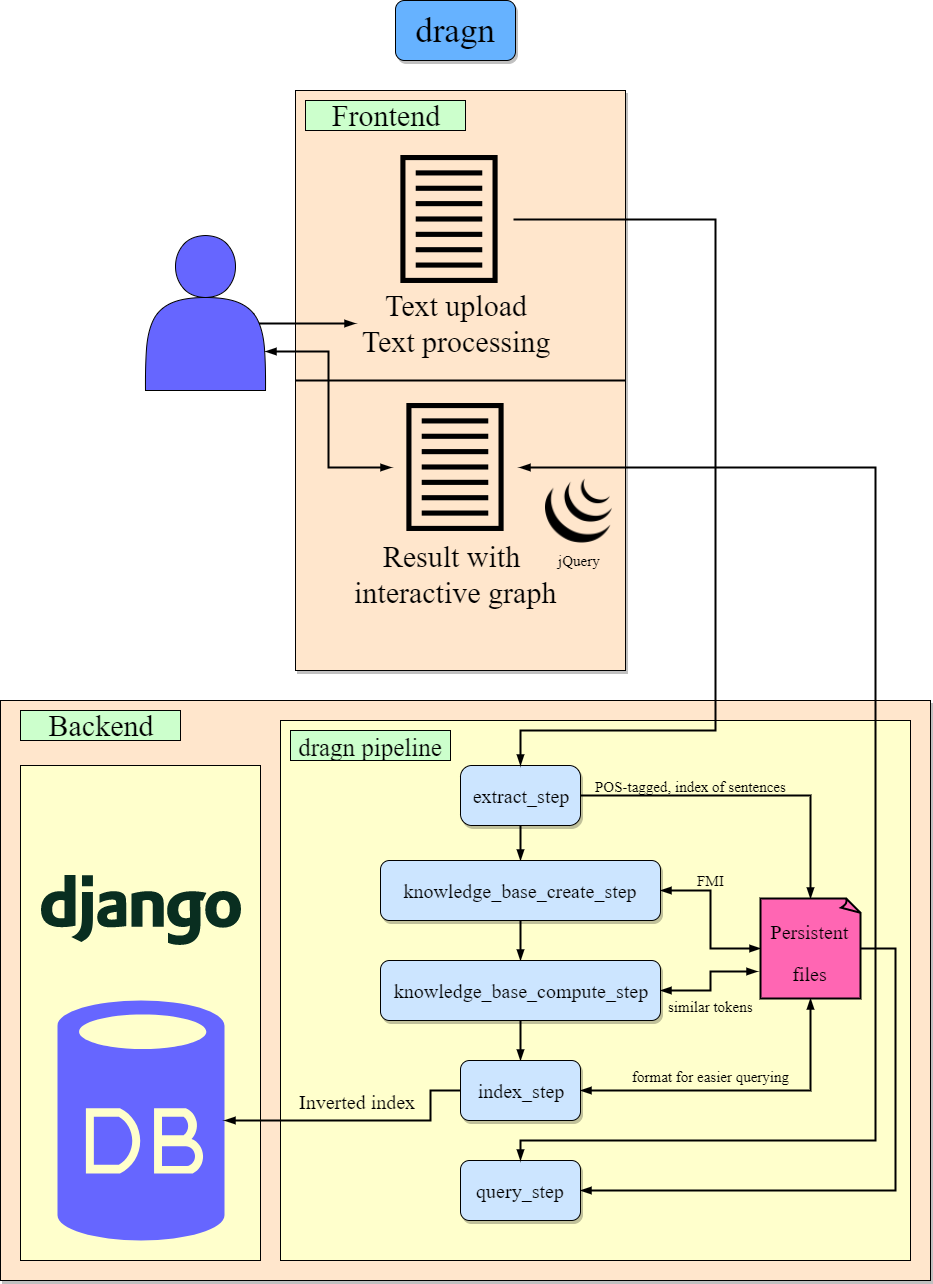
\includegraphics[scale=0.53]{fig/dragn_structure1_1}
    \caption{Overview of "dragn" system architecture}
    \label{fig:dragn_overview}
\end{figure}

%%=========================================
\section{Architecture Overview}\label{overview}
The original system, Skimmr \cite{novavcek2014skimmr} is written in Python 2.7, whereas \textbf{dragn} is written in Python 3.5. The main "support" framework of the system is Django 1.10.6, which is mostly used to lessen the burden on the user when setting up the system on a network and to easily provide an interactive interface to the user. The system was built with the deployment on a (research) network in mind to allow multiple people to use it for work at once.\\
For the interaction part specifically, another framework is used: \textit{Cytoscape.js} \cite{doi:10.1093/bioinformatics/btv557}. It allows the display of graphs from JSON (Javascript Object Notation) data and supports exporting the result graphs as JSON as well, allowing users to use the results more easily in complex ways.\\
The core of the system is built upon four steps (five if including the queries):
\begin{itemize}
    \item extract\_step - Extracts paragraphs and tokens from texts, applies POS-tags and builds an inverted index of sentences.
    \item knowledge\_base\_create\_step - Calculates a modified PMI, the FMI, (for more details, see chapter \ref{sec:fmi}) over all tokens in the texts.
    \item knowledge\_base\_compute\_step - Calculates Cosine Similarity over tokens from the texts using the FMI values.
    \item index\_step - Brings the results of the previous two steps in a more easily accessible format.
    \item query\_step - Performs the user's queries on the data and produces a graph in JSON format for use with \textit{Cytoscape.js}.
\end{itemize}
Texts are uploaded into the system through the web interface, afterwards the texts to process are selected. For this, the \textit{Alias System} is used: A combination of texts is processed together and this combination of texts can be selected from a dropdown when performing a query. The name in the dropdown is an alias for the bundled texts, hence the name, and this bundling persists. An arbitrary number of aliases can exist at once, allowing the user to select which combination of texts to query.\\
While the texts themself are stored directly on the disk, the aliases and their corresponding texts are stored in the Django database.\\
Overall, the system follows the MVC (Model-View-Controller) pattern, with the HTML front end and Django embodying the View and Controller respectively, while the system's back end with the \_step pipeline is the Model part of the pattern.\\
MVC is an important pattern used commonly in Software Engineering and using it gives the system greater flexibility regarding the display of the results and data, as an integral part of the MVC architecture is to have the user interface be completely replaceable without having to modify the core of the system.

%%=========================================
\subsection{Use of Django}
Django is used because of its widespread use and ease of setup on different systems. More specifically, the HTML pages are served by Django and its internal templating engine. The database integration of Django is used for the Alias System and for the inverted index.
%%=========================================
\subsection{Inverted Index}
An inverted index is the mapping of text fragments, generally processed words in a text, to a list of texts they appear in. As an example:
\begin{table}[h!]
\centering
\caption{Example inverted index}
\label{table:inverted-index}
\begin{tabular}{l|l}
Token & Documents \\ \hline
apple & story.txt, story2.txt, story2.txt \\
tree & story2.txt, story3.txt, story49.txt 
\end{tabular}
\end{table}
For this inverted index, \textit{apple} appears in documents \textit{story.txt}, \textit{story2.txt} and \textit{story2.txt7}.\\
Data structured in this way allows easy and quick access to texts containing certain words.\\
In \textbf{dragn}, such an index is used to bolden all tokens appearing in paragraphs relevant to the query that also appear in the result graph. For more details, see chapter \ref{sec:resultgraph}.

%%=================================
\subsection{Alias System}
\label{sec:alias}
\textbf{dragn} works by passing it collections of texts which the system then processes into files that are used to satisfy the user's queries. Due to the nature of the system, it is very likely that the user might want to analyse permutations of their corpus. To support that need, the \textit{Alias System} was implemented.\\
Before the user can work with the system, the texts that are going to be the base for the queries have to be uploaded to the system and selected. The selected combination of texts is assigned an \textit{Alias} in the system and an entry in the database is added to map the Alias to the names of the texts. This is then used by the system to identify which files belong to which combination of texts by having the files written to folders named after the Alias.\\
When performing a query the user can then select the Alias from a list and query only the texts belonging to that Alias. The Aliases and the files created during the processing of the texts persist between queries and thus the user can at any time decide to work with a specific subset of their texts by selecting the corresponding Alias and performing a query.\\
By default, the name of the Alias is a combination of the file names to lessen the burden of knowledge on the user, but any other presentation is possible.\\
An example:
\begin{table}[h!]
\centering
\caption{Example of the Alias System}
\label{table:alias-example}
\begin{tabular}{l|l}
Alias & Documents \\ \hline
story.txt,story2.txt & story.txt, story2.txt \\
story.txt & story.txt
\end{tabular}
\end{table}
\\
In this example based on table \ref{table:alias-example}, the user can select "story.txt" as the Alias and perform queries on the processed files of the document "story.txt" without having to make the system process the text beforehand, because that has already been done.\\
The Alias System is especially advantageous when multiple users are working with the system. Previously processed permutations of texts created by other users are selectable as an Alias and can immediately be queried.\\
Due the separation of processed files into different sub-directories as per their Alias the individual permutations queries on a specific Alias experience no slowdown from the other Aliases, as would be the case without a separation into multiple files. In that case, either a single massive file would have to be loaded and the relevant upshot of the previous processing of files be filtered out to get only the content relevant to the current texts or complex database queries doing the same would need to be performed.\\
The core of the system is to find information like "apple is connected to tree", but to also allow the user to understand why that connection has been found and where this connection becomes apparent in texts. However, the user might be interested to see the connections of a certain word to other words in a single or multiple specific texts and compare them. "Apple" might appear often near "tree" in a botanical text and have a high PMI, but in a different text their PMI might be low.\\
In \textbf{dragn} this problem is accounted for by producing multiple files containing such information and having those files be mapped to an Alias of either a single text or multiple texts together.\\
Without the Alias System the files of a previous processing would either have to be deleted and thus the texts would have to be processed again later, or a very complex system would have to be built to contain and extract the information for multiple texts from the files.\\
The Alias System circumvents this problem and is an integral part of the system's usability.
%%===================================
\section{Extraction of Noun Phrases and calculation of distance}
\label{sec:extract}
The following chapters are intended to give a detailed insight into the different parts of the system, how they work individually and how their outputs are used in the consecutive steps.\\
This chapter aims to provide the reader with a comprehensive understanding of the first step in the \textbf{dragn} pipeline, \textit{extract\_step}.\\
As briefly touched upon in the previous chapter \ref{sec:alias}, each of the four main steps of the \textbf{dragn} pipeline produces persistent files that are contained in folders named after the Alias of the texts. The folders for those files are created as part of this first step and the uploaded texts are moved into the corresponding directory.\\
The texts are then processed one by one. Initially, the paragraphs are extracted from the texts. They are part of the result of the queries, paragraphs containing words relevant to the query (see \ref{sec:querystep}). The system operates under the assumption that paragraphs in a text are logical, self-contained units and as such the system works on a per-paragraph basis. A clarification with an example will follow shortly.\\
Next is the POS-tagging of the sentences in the current paragraph. POS stands for "Part Of Speech" and tagging words in such a way means to assign labels such as "Noun", "Proper Noun", "Adjective". The tagset used is the Penn Treebank \cite{marcus1993building}. Grammatical inconsistencies may exist in text, especially if it is not a properly published work where editors are proofreading, but generally it can be assumed that the grammar is correct enough to properly label the parts of the sentences.\\
The POS-tags are useful because they allow for the extraction of Noun Phrases from the sentences. For this extraction, grammar from the original system developed by \cite{novavcek2014skimmr} is used. This grammar, combined with parsers from NLTK (Natural Language Toolkit) is used by the parser to find Noun Phrases. Noun Phrases are concatenated words in a text that describe a single entity, such as \textit{yellow dog}, as described in \cite{abney1987english}.\\
Two grammars for the English language are currently in the system, developed by \cite{novavcek2014skimmr}.
\begin{lstlisting}[frame=single, caption={Noun Phrase grammars}, label=npgrammar]
NP_GRAMMAR_COMPOUND = """
NP: {
        <JJ.*>*(<N.*>|<JJ.*>)+
        (
            (<IN>|<TO>)?<JJ.*>*(<N.*>|<JJ.*>)+
        )*
        (
            (<CC>|,)<JJ.*>*(<N.*>|<JJ.*>)+
            (
                (<IN>|<TO>)?<JJ.*>*(<N.*>|<JJ.*>)+
            )*
        )*
    }
"""
NP_GRAMMAR_SIMPLE = """
NP: {<JJ.*>*(<N.*>|<JJ.*>)+}
"""
\end{lstlisting}
Note that \textit{NP\_GRAMMAR\_COMPOUND} has been split into multiple lines for easier readability in this thesis at the cost of not being valid for use in Python anymore. The correct grammar is a single line which makes it harder on the reader to understand what is happening and is of course still included as such in the source code of the system.\\
The purpose of the grammars is to extract Noun Phrases from the texts.\\
First the POS-tagged sentences for each paragraph of a text are chunked using the \\
\textit{NP\_GRAMMAR\_COMPOUND}. An explanation with an example of NP-chunking and the role of grammars will now be discussed to help the reader understand the following parts.
\subsubsection{NP-chunking and grammars}
Generally speaking the goal of NP-chunking is to find Noun Phrases in texts. Consider the following sentence:
\begin{lstlisting}
The/DT little/JJ yellow/JJ fruit/NN outside/IN Passau/NNP.
\end{lstlisting}
The letters after each word are the word's corresponding POS-tag.\\
For this sentence it makes sense to consider \textit{little yellow fruit} as a Noun Phrase. \textit{fruit} is clearly a noun and \textit{yellow} and \textit{little} refer to the fruit. To combine those words into a single Noun Phrase we use the grammar from above.\\
In the first line we have
\begin{lstlisting}
<JJ.*>*(<N.*>|<JJ.*>)+
\end{lstlisting}
which can be read as:
\begin{itemize}
\item zero or more adjectives (the Penn Treebank POS-tags for adjectives all begin with JJ, hence the JJ.*, see \cite{PennTreebank})
\item ... followed by either one or more (the + means one or more, it applies to whatever is inside the brackets):
    \begin{itemize}
    \item a noun (the POS-tags for nouns all start with N, hence the N.*)
    \item another adjective
    \end{itemize}
\end{itemize}
Therefore, by reading the tags in the example sentence given, we see that \textit{little yellow fruit} follows the rules and thus would be a Noun Phrase according to the grammar.\\
As we read the next line, we have the continuation of the grammar:
\begin{itemize}
\item zero or more of (the asterisk at the end of round bracket) the following construct:
    \begin{itemize}
    \item exactly one of either (the question mark means zero or one times)
        \begin{itemize}
        \item preposition or subordinating conjunction
        \item the word "to"
        \end{itemize}
    \item followed by any number of adjectives
    \item followed by one or more of either:
        \begin{itemize}
        \item a noun
        \item an adjective
        \end{itemize}
    \end{itemize}
\end{itemize}
We continue to read the sentence and see that \textit{outside Passau} satisfies this next line of the grammar. Therefore \textit{little yellow fruit outside Passau} is a Noun Phrase we extracted from the sentence using the compound grammar.\\
The two lines that were omitted for this example work in exactly the same way, the Noun Phrases we can extract would simply be longer and more complex.\\
\subsubsection{Usage of the extracted Noun Phrases in dragn and distance calculation}
In \textbf{dragn} the grammars are used to extract the Noun Phrases from each sentence. As the system processes each paragraph for each text individually, we have access to the sentences and can use them to map the extracted Noun Phrases to the sentences they appear in to create what is essentially an inverted positional index. As Noun Phrases can be made up of multiple words, they allow the user to more finegrainedly perform queries, instead of simply searching for "fruit" it becomes possible to search for "red fruit" as an example. Extracting Noun Phrases makes it possible to search for relations only between Noun Phrases and find more specific relations, such as "apple IS A red fruit". For more details, refer to the suggestions for further work in chapter \ref{sec:furtherwork}.
\begin{table}[h!]
\centering
\caption{Inverted positional index}
\label{table:inverted-posindex}
\begin{tabular}{l|l}
Lexical unit (for example Noun Phrases or just single verbs) & Sentence position in paragraph \\ \hline
little yellow fruit & 0, 2, 3 \\
apple & 0\\
rocket & 20\\
\end{tabular}
\end{table}
\\
As the overall goal is to find tokens in text that are related to each other in some way, it is a good idea to filter out combinations that are very unlikely to be linked. Consider the simple Noun Phrases "apple", which appears in the first sentence, and "rocket", which occurs twenty sentences later (see table \ref{table:inverted-posindex}). A semantic link between those two words is very unlikely due to their distance in sentences. For that reason, a weighted distance score is calculated.\\
The general idea behind this is that words that are very far apart are unlikely to be related. Therefore, we use the positional index that was created while extracting the Noun Phrases to filter out pairs that cannot be related.\\
Calculating the score is simple. For each combination of lexical units from the positional index, we look at all the positions of the two where the distance is below five sentences. If the distance is too big, for example ten sentences, they are very unlikely to be related. We continue with the calculation of their weighted distance, which is \(w += 1/(1 + distance\). The further apart they are, the lower the update to their weighted distance. If their weighted distance is above the threshold of \(1/3\) the pair is added to a list for further processing in the next step, where the PMI between the two is being calculated.\\
For the data in table \ref{table:inverted-posindex} we would thus get the following result for \textit{apple} and \textit{little yellow fruit}:
\begin{equation}\label{gather:weighteddistance}
\begin{aligned}
w &= \frac{1}{1+0} = 1 \text{ (positions 0 and 0)} \\ 
w &+= \frac{1}{1+2} = 1 + 0.333 = 1.333 \text{ (positions 2 and 0)}\\
w &+= \frac{1}{1+3} = 1.333 + 0.25 = 1.583 \text{ (positions 3 and 0)}\\
\end{aligned}
\end{equation}
It is easy to see that the higher the distance, the lower the change to the weight becomes. Important to note here is that tokens which appear consistently multiple sentences apart would have a score higher than the threshold and be considered. In that case, a relation between the two might be possible and the system keeps them to have their PMI calculated.

%==============kb create
\section{Calculation of modified PMI between words - FMI}\label{sec:kbcreate}
In this step the modified PMI is calculated over the units from the texts. The basis for that are the extracted \textit{<token> close to <token2>} triples calculated as per chapter \ref{sec:extract}, from here on referred to as SPO- or \textit{Subject-Predicate-Object} triples as per the naming conventions in the original system developed by \cite{novavcek2014skimmr}. If their textual origin, the \textit{provenance} is included, they will be referred to as \textit{SPOP-tuple}.\\

%====pmi subjection
\subsection{FMI - PMI with emphasis on the frequency and weighted distance}
\label{sec:fmi}
As mentioned before, the system does not use the classic Pointwise Mutual Information or PMI but a modified one as developed by Vit Novacek. In this chapter, first that modified PMI is explained and then the differences to the classic PMI highlighted. \\
An approach similar to the one in this thesis is used in \cite{recchia2009more} to compare PMI and LSA \cite{landauer2006latent}. The approach discussed therein uses a model based on word counts whereas in this thesis the distance between two words is used.
In \cite{church1990word}, the PMI is defined as:\\
\begin{gather}
\label{formula:pmi}
    \operatorname{PMI}(x;y) \equiv \log[2][]{\frac{p(x,y)}{p(x)p(y)}}
\end{gather}
It is used to measure statistical independence between two outcomes \textit{x} and \textit{y}. A positive PMI means the two outcomes co-occur more often than would be expected by chance, so therefore a connection between the two can be assumed, and a negative PMI means they co-occur less often than would be expected. A score of zero means they are independent \cite{bouma2009normalized}.\\
We take the probability of the two outcomes co-occurring and divide it by the probability of them simply occurring by chance (refer to \cite{church1990word}, p. 2, chapter 4).\\
As a simple example, \textit{apple} and \textit{tree} would have a high PMI in a text about an orchard. For the sake of this example, assume they are dependant on each other. The occurrence of the fruit is closely tied to the word \textit{tree}.\\
The PMI is a useful measure because we can calculate how dependant the appearance of a phrase or word in a text is on the appearance of another phrase or word. A modified PMI that takes into account the average weighted distance calculated as in \ref{gather:weighteddistance} and emphasises the frequency more strongly is used in this system. The original concept behind this was developed and defined by Vit Novacek \cite{novavcek2014skimmr}.\\
\begin{gather}
\label{formula:fmi}
  \operatorname{FMI}(p1;p2) \equiv joint(p1, p2) *
    \log[2][]{\frac{\#relations * (joint(p1, p2) + joint(p2, p1)}{\#p1 * \#p2}} * \frac{\sum{}{distances}}{\#distances}\\
    \text{With} \operatorname{joint}(p1, p2) \equiv \text{Number of relations with "p1 close to p2"}
\end{gather}
First the equivalence between the middle part (the log) and the PMI formula will be shown. In the context of this system we look at the relations that were calculated in the first step \ref{sec:extract} and check in how many of them the phrases or words we are calculating the PMI for appear.

\begin{align*}
\label{formula:equivalence}
\operatorname{PMI}(p1;p2) &= \log[2][]{\frac{\frac{y}{x}}{\frac{z}{x} * \frac{w}{x}}} \\
\end{align*}
Where
\begin{align*}
~y &= \text{number of relations with both p1 and p2}\\
~x &= \text{number of relations}\\
~z &= \text{number of relations with p1}\\
~w &= \text{number of relations with p2}\\
~p1/p2 &= \text{words or phrases from a text}
\end{align*}
By inserting those into the PMI formula we get:
\begin{align*}
\operatorname{PMI}(p1;p2) &= \log[2][]{\frac{\frac{y}{x}}{\frac{z}{x} * \frac{w}{x}}} =\\
                          &= \log[2][]{\frac{\frac{y}{x}}{\frac{zw}{x^2}}} =\\
                          &= \log[2][]{\frac{yx^2}{xzw}} =\\
                          &= \log[2][]{\frac{xy}{zw}}\\
\operatorname{FMI}(p1;p2) &= \log[2][]{\frac{\#relations * (joint(p1, p2) + joint(p2, p1)}{\#p1 * \#p2}} = \\
    &= \log[2][]{\frac{x * y}{z * w}} = \\
    &= \operatorname{PMI}(p1;p2)\\
\text{Therefore}\\
\operatorname{FMI}(p1;p2) &= joint(p1, p2) * \operatorname{PMI}(p1;p2) * \frac{\sum{}{distances}}{\#distances}
\end{align*}
We thus see the FMI formula is just the PMI formula but with the average weighted distance and the frequency added. \\
An example will now be calculated to show how the formula works: Consider the following data:
\begin{table}[h!]
\centering
\caption{Example result of extract\_step}
\label{table:extract-example}
\begin{tabular}{l|l|l|l}
Extracted phrase / token & Phrase / Token that will be checked & Weighted distance & Provenance\\ \hline
apple & roof & 1.2 & story.txt\_1\\ \hline
tree & apple & 0.8 & story.txt\_1\\ \hline
apple & tree & 0.6 & story.txt\_2 \\ \hline
\rowcolor{grey!25}tree & leaf & 1.3 & story.txt\_2 \\ \hline
tree & roof & 0.7 & story.txt\_1
\end{tabular}
\end{table}\\
The first line in table \ref{table:extract-example} means "apple" has a weighted distance (\ref{gather:weighteddistance}) of 1.2 to "roof" in \textit{story.txt\_1}, which itself means "the first paragraph of the file story.txt".\\
We will use "tree" and "leaf" as the example for the calculation.\\
\begin{equation}\label{gather:fmiexample}
\begin{aligned}
\operatorname{PMI}(tree;leaf) &= \log[2][]{\frac{\frac{1}{5}}{\frac{4}{5} * \frac{1}{5}}} = 0.3219 \\
\operatorname {FMI}(tree;leaf) &= 1 * 0.3219 * \frac{1.3}{1} = 0.70
\end{aligned}
\end{equation}
\textit{joint(p1;p2)} is always positive, if there is no co-occurrence then calculating the PMI or FMI makes no sense. The same applies for a negative joint value, in the context of co-occurrences in a text this can never happen.\\
Now consider the average weighted distance. This value too can never be negative or zero. It can be lower than 1, in which case the FMI would be lower than the PMI value. This would be the case if the weighted distance between "tree" and "leaf" was not 1.3 but 0.8 for example. A low weighted distance means the distance between the two words or phrases is high.\\
We can therefore see that the modified PMI value, the FMI, rewards words co-occurring in different paragraphs, but consistently. The more paragraphs they co-occur in, the higher the joint frequency multiplier. On the other hand, it punishes high distance in the co-occurrences, the higher the distance the lower the weighted distance and the lower the average weighted distance multiplier.\\
This modified FMI is useful precisely because of those properties. The PMI does not consider the distance at all, it uses a binary measure to count how often two events co-occur (the events here being words or phrases co-occurring in a text). This is not good enough. Words that appear very close together, very often, are likely more related to each than words that appear together, but far apart. In the worst case two words co-occur in many different paragraphs consistently, but far apart. With the normal PMI measure they would have the same score as a pair of words that appears directly after each other in the same paragraphs. However one would expect that words that appear consistently close to each other are more related to each other than those consistently far apart from each other. The FMI formula discussed in this chapter scores the closely co-occurring words higher while still keeping the expressiveness, whether two events occur more frequently together than apart, in this context appearing together in a text, of the PMI formula and is thus a good measure to use in the context of Distant Reading. We can query for words that we know occur in a text from the context or title and find other words or phrases that appear near it and thus gain additional information about the text with minimal effort.

%=====usage of PMI in dragn
\subsection{Normalisation of the FMI values}
The extracted weighted distances as described in chapter \ref{sec:extract} are used to calculate the FMI values as described in the previous chapter \ref{sec:fmi}. The result is a dictionary mapping the SPO-triples to their FMI score. \\
The calculated FMI values are then normalised. For that, the SPO-triples are sorted by their FMI value. The lowest value of the 5\% of top FMI scores is then used as the normalisation value. The values are all normalised to a value between a minimum value, default being 0.1, and 1 as the upper limit. The normalisation performed is a simple division of the FMI value by the normalisation value.\\
This procedure results in lower normalised FMI values for the bottom 95\% of values and a higher normalised value for the top 5\%. This is intentional to have the top values be weighted even higher. Doing this emphasises those top results more when performing the query.\\
The normalised values are then written to the disk with the help of the Alias System as shown in chapter \ref{sec:alias} and used to calculate the words or phrases that are related to another word or phrase not directly through their FMI value, but through co-occurrence of of a word or phrase that has a high FMI value with the original.\\
The calculated triples are written to the disk and then used to build a vector space and calculate the Cosine Similarity in the next step.

%=======kb compute
\section{Calculation of Cosine Similarity based on FMI values}
\label{sec:kbcompute}
The goal of this step is to compute tokens or phrases that are \textit{related to} another token or phrase. Note that \textit{related to} refers specifically to the relation calculated over the vector space of the SPO-triples, their similarity to be exact. The exact process will be explained in this chapter, but first that vector space must be built.\\
The \textit{close to} SPO-triples calculated with their FMI in the previous chapter \ref{sec:kbcreate} are loaded in using the Alias System \ref{sec:alias}. Then a sparse matrix representation of those triples is calculated. A sparse matrix is a matrix in which most elements are zero.\\
\begin{table}[h!]
\centering
\caption{Example sparse matrix}
\label{table:sparse}
\begin{tabular}{l|l|l|l|l}
 & apple & tree & leaf & fruit\\ \hline
apple & 0 & 0.9 & 0.5 & 0 \\ \hline
tree & 0.9 & 0 & 0.6 & 0\\ \hline
leaf & 0.5 & 0.6 & 0 & 0.4 \\ \hline
fruit & 0 & 0 & 0.4 & 0\\ 
\end{tabular}
\end{table}\\

It is constructed by iterating over the SPO-triples we calculated in the previous step. The way the matrix as represented in table \ref{table:sparse} is read is as follows:\\
\centerline{tree is close to leaf with an FMI value of 0.6 (row 3)}\\


\subsection{Cosine Similarity and its role in dragn}
The Cosine Similarity for two vectors x and y is given by:
\begin{flalign*}
\label{formula:cosine}
cos(x,y) = \frac{x \cdot y}{|x|\cdot|y|}
\end{flalign*}
Where
\begin{flalign*}
x = (x_1, x_2, ... x_n)^\intercal\\
y = (y_1, y_2, ... y_n)^\intercal\\
\end{flalign*}
are vectors in an n-dimensional vector space and 
\begin{flalign*}
|x| = \sqrt{x_1^2 + x_2^2 + ... + x_n^2}
\end{flalign*} is the length of the vector, as discussed in \cite{singhal2001modern} and \cite{rahutomo2012semantic}.\\
Simply put, the cosine of the angle between two vectors is used to compare the similarity between the vectors. The lower the angle the more similar the vectors are.\\
Continuing the example from above, the rows in table \ref{table:sparse} are vectors in the vector space over the processed texts.
We can compute the similarity for "apple" and "tree" based on their respective FMI values with other words in the table.\\
\begin{flalign*}
x_y = \text{FMI value for x with y}
\end{flalign*}
Then we calculate the lengths of the "tree" and "apple" vectors:
\begin{flalign*}
|tree| &= \sqrt{tree_{apple}^2 + tree_{leaf}^2} = \sqrt{0.9^2 + 0.6^2} = 1.08\\
|apple| &= \sqrt{apple_{tree}^2 + apple_{leaf}^2} = 1.030
\end{flalign*}
Next we calculate the product of the two rows in table \ref{table:sparse}:
\begin{flalign*}
\overrightarrow{tree} \cdot \overrightarrow{apple} &=
    tree_{apple} * apple_{apple} + tree_{tree} * apple_{tree} + tree_{leaf} * apple_{leaf} + tree_{fruit} * apple_{fruit}\\ &= 0.9 * 0 + 0 * 0.9 + 0.6 * 0.5 + 0 * 0 = 0.6 * 0.5 = \\
    &= 0.3
\end{flalign*}
We insert those values into the Cosine Similarity formula and get:
\begin{flalign*}
cos(tree,apple) = \frac{0.3}{1.08 * 1.03} = 0.270
\end{flalign*}
Therefore the Cosine Similarity based on the FMI values is 0.270, which is on the lower side. The Cosine Similarity values range from 0 to 1, with 1 indicating there is no angle between the two vectors, thus showing they are pointing in the same direction in their vector space. \\
Let
\begin{flalign*}
x = (x_1, x_2, ..., x_n)^\intercal\\
y = (y_1, y_2, ..., y_n)^\intercal\\
x = y
\end{flalign*}
then
\begin{flalign*}
|x| = \sqrt{x_1^2 + x_2^2 + ... + x_n^2} = \sqrt{y_1^2 + y_2^2 + ... + y_n^2} = |y|
\end{flalign*}
\begin{flalign*}
|x| * |y| = |x|^2 = x_1^2 + x_2^2 + ... + x_n^2
\end{flalign*}
\begin{flalign*}
cos(x, y) &= \frac{x_1 * y_1 + x_2 * y_2 + ... x_n * y_n}{|x|*|y|} = \\
&= \frac{x_1^2 + x_2^2 + ... + x_n^2}{x_1^2 + x_2^2 + ... + x_n^2} = 1
\end{flalign*}
Therefore for two tokens that have the exact same FMI values and thus co-occurrences with the same distances their similarity value will be one, indicating they are functionally identical in this context.\\
The Cosine Similarity can be used to calculate similarity between documents as described in \cite{singhal2001modern}, however as shown in this chapter one can calculate the similarity between vectors of FMI values. The result we get here is a similarity score calculated between two phrases or words in a text, based on their FMI values, which as explained in chapter \ref{sec:kbcreate} is based on the co-occurrence of phrases in a text. The Cosine Similarity in this context is therefore grounded in the co-occurrence of two phrases not with each other, but with tokens in texts they both co-occur with. Their similarity increases \\
A similarity scoring function is useful in the context of Distant Reading, for given words appearing in texts we want to find words or phrases that are related in some way. This system makes the assumption that words with word vectors pointing in similar directions (thus having a high Cosine Similarity) are related to each other. For their similarity to be high, they need to have high FMI for the same words. In simpler terms, if two words co-occur often with the same words but not each other, the assumption is made that they are related.\\
The FMI value that is used as the score value for the similarity computation connects two phrases or words when they co-occur in a text. By using those values as the basis for the calculations we can find phrases that are similar by checking which words they share a high FMI value with, or in other words, how big the angle between the two vectors of FMI values is.\\
Ultimately we find phrases that share common FMI values. If a word co-occurs with other words often, and a second word co-occurs with the same words and a comparable frequency, we establish a relation between the two with the method discussed in this chapter. Those two words appear near the same words often, so we can assume the two words themselves are related. This gives us a less-intuitive way of finding connections between words in texts, that would be hard to accomplish by hand.\\
We now have useful information that we could query and gain information about texts from. To do that, the following chapter shows how the produced files are formatted and written to new files that can be used as the basis for the queries or used in a different system.

\section{Creation of formatted files / index}
\label{sec:indexstep}
The ability to expand and build upon \textbf{dragn} is one of the core goals of the overall design of the system. In the previous chapters the algorithms and calculations performed in the system were outlined, all that is left is bringing the data in a form that is easier to query. In this chapter I will show how the different files for the queries are created and in which format they are. It is then possible to use the results produced in \textbf{dragn} for other systems but with a different scope or use.\\
The subsection titles refer to function names in the system.
\subsection{Creation of SPO-triples list}
\label{sec:makerelationlist}
First the SPOP-tuples as created in chapter \ref{sec:kbcreate} are loaded. They are in the format:
\begin{align*}
    \text{<subject> <predicate> <object>, score}
\end{align*}
Where \textit{subject} and \textit{predicate} are words or phrases from the texts that the system found a relation between, and \textit{predicate} is one of \textit{close to} for the FMI relations or \textit{related to} for the similarity relations.\\
All the relations that were found for the current text(s) are written to a file on the disk.\\
The format is, where \textit{\\t} is the tab character:
\begin{lstlisting}
subject\tpredicate\tobject\tscore
\end{lstlisting}
By loading this file and parsing the data one can have access to all the relations that were calculated over a set of texts. The Alias System as outlined in chapter \ref{sec:alias} makes it possible to keep the files created for collections of texts and compare the results, as an example usage.

\subsection{Creation of SPO shortlist}
\label{makerelationweights}
In this file,  the subject, object and score of the SPOP-tuples are saved in the format:
\begin{lstlisting}
subject\tobject\tscore
\end{lstlisting}
The contents of this file can be used to quickly find which words have a relation between them and with what value. Due to the reduced content of the file it is smaller and can be loaded faster, which becomes increasingly more relevant with the number and size of the processed texts.


\subsection{Creation of SPOP-tuples list}
\label{sec:relationmapping}
The first part of this function is to create an inverted index over the processed texts. This index is used in the following chapter to improve the information value of the query results.\\
The second and main purpose of this function is to map SPO-triples to their score in provenances.\\
The format is:
\begin{lstlisting}
(subject, predicate, object)\t[(provenance, score)]
\end{lstlisting}
The "related to" triples are added separately to get a text-specific set of relations. We do that by iterating over all the "related to" triples we have to get all the relations with them and to know the provenances they belong to. We iterate over all "related to" triples and for the subject and object of the relations we find the relations they have in common.\\
For those extracted relations two new triples are built:\\
\centerline{subject predicate object-from-commons}\\
\centerline{object-from-commons predicate object}\\
Where \textit{object-from-commons} is the object of the (relation, object) tuple. The tuples are mapped against the word they have a relation with, so one can access all the relations a word or phrase has and finds a list of the tuples described.\\
\begin{lstlisting}[caption=Example relation mapping for "apple"]
mapping = {
    "apple": [(close to, tree), (related to, leaf)]
}
mapping["apple"] = [(close to, tree), (related to, leaf)]
\end{lstlisting}
For those new triples the mapping of triples to (provenance, score) tuples is checked and for each of the provenances the maximum score is extracted, then we add a line in the known format:\\
\textit{subject predicate object, provenance, score}\\
Where score is updated to be:
\begin{lstlisting}
score = original\_triple\_score * new\_triple\_score
\end{lstlisting}
and subject or object respectively replaced with the object from the (relation, object) tuple.\\
This results in artificial "related  to"-triples that exist in provenances.
An example of the usage:\\
\textit{apple related to tree, 0.8} is the triple we look at.
We find:
\begin{lstlisting}
relations[apple] = (close to, fruit)
relations[tree]  = (close to, fruit)
\end{lstlisting}
\textit{close to fruit} is found in the relations for both \textit{tree} and \textit{apple}. Therefore we check the two triples:
\begin{lstlisting}
apple close to fruit (we keep the subject from the original triple)
tree close to fruit (we keep the object from the original triple)
\end{lstlisting}
We now look up the triple-provenance mapping and find the following:
\begin{lstlisting}
provenance_mapping[(apple close to fruit)] = (story1_1.txt, 0.6)
provenance_mapping[(tree close to fruit)]  = (story1_1.txt, 0.7)
\end{lstlisting}
The maximum score for story1\_1.txt is 0.7 for the triple "tree close to fruit", which is the triple where we kept the object. That means we keep the original object and replace the subject with \textit{fruit} and get:
\begin{lstlisting}
fruit related to tree, story1_1.txt, 0.8*0.7
\end{lstlisting}
We thus can say that \textit{fruit is related to tree in the text story1\_1.txt with a score of 0.56}. This was created because we have the original relation \textit{apple related to tree} and \textit{fruit} appears near both \textit{apple} and \textit{tree} in the same paragraph, so we augment the data by adding this new relation \textit{fruit related to tree}.

\subsection{Summary of the indexing}
In this chapter I have shown how the calculated data is augmented to improve results and how it is brought into formats that are easier to use with my own system but also to use with other systems. For that reason the structure of the data was explained, thus enabling the reader to use the data in their own work easily.\\
This step is rather complex from a programming and understanding standpoint.The reader is encouraged to use this chapter and the files created in this step for their own project or research.\\
Now that the files are all processed and in place, all that is left is to perform queries. The usage of the files created in this chapter and their role in the queries will be shown in the following chapter and the last step.

\section{Calculation of query results}
\label{sec:querystep}
This chapter will explain how queries are answered in \textbf{dragn}. The implementation shown here is just an example, the data output outlined in chapter \ref{sec:indexstep} can be used in different ways and for different projects. In this chapter however the output of the previous chapter will be used as is. \\

\subsection{Calculation of relevance to the query}
\label{sec:popdict}
First a \textit{Fuzzy Set} over all relations that contain a query term is calculated using the mapping of tokens to their contained relations, see chapter \ref{sec:makerelationlist}. The original implementation of the fuzzy sets and the idea to use them in this way come from Vit Novacek \cite{novavcek2014skimmr}.\\
Whereas a "normal" set has a binary relation to its contained elements (an element is either part of the set or not) a fuzzy set has a degree of membership, as introduced in \cite{zadeh1965fuzzy}.\\
Calculating a fuzzy set in the context of the system and specifically the query results in a fuzzy set describing how high the membership of a token to the query is.\\
If a query contains more than one query term and terms share a relation but with different scores, the higher of the scores is used as the membership.\\
All relations (= SPO-triples) containing members of this fuzzy set and a query term are then checked one by one. The score of the SPO-triples is then multiplied by the membership from the fuzzy set.\\
This increases the score of low-scoring relations if the complementary relation has a higher value and decreases the scores overall. A high degree of membership increases the score in comparison to low membership.\\
A dictionary then holds the score we just calculated for subject and object of the SPO-triples, the same steps are performed for all relations containing fuzzy set member and a query term. The result is a dictionary mapping tokens to a score, the tokens sorted by their score will become the result of the query later.\\
Additionally the provenances for the SPO-triples are loaded from the mapping (see \ref{sec:relationmapping}) and the multiplication of membership and score is performed again as above. This score and the triple are then likewise mapped to each provenance.\\
With this relatively simple calculation out of the way it is now possible to create a graph showing relations between tokens from the texts and the query terms and show relevant text samples. This will be discussed in the following chapter.

\subsection{Graph generation and the dragn graph system}
\textbf{dragn} uses its own, simple graph system with three parts:
\begin{itemize}
\item \textbf{Nodes}\\
    They have a name and width and colour. A container for Edge objects.
\item \textbf{Edges}\\
    They have a start and an end, which can be anything. Intended for them to be Nodes. 
\item \textbf{Graph}\\
    A graph is a container for nodes.
\end{itemize}
Important here is that the graph system is very simply built and easily extendable. The main purpose of it is to generate RFC4627 compliant JSON, as described in \cite{crockford2006application}. The simplistic nature allows for the creation of any kind of graph that can be exported to JSON very easily.\\
In \textbf{dragn} the graphs are created from the data in the previous chapter, \ref{sec:popdict}. A maximum number of nodes is created based on the sorted scores. Each node represents a token or phrase from the processed texts. If the node label appears in the query, the node is coloured differently to make it easier for the user to find what they are interested in.\\
After the nodes are generated, all the relations are checked. If both subject and object appear as a node, an edge is created between them, with the colour showing their relation, up to a maximum number of edges as specified by the user.


\section{dragn interface}
This section contains a short explanation and summary of the \textbf{dragn} user interface.

\subsection{Navigation bar}
\label{subsec:navbar}
The navigation bar is where the user enters the information for their query. It contains buttons to go to the pages for text upload and text processing.
\begin{figure}[H]
    \centering
    \hspace*{-1,5cm}
    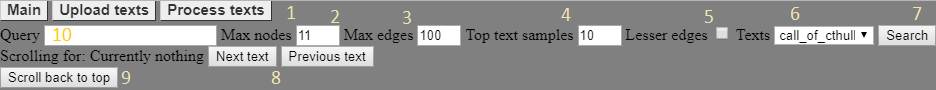
\includegraphics[scale=0.8]{fig/search-interface}
    \caption{Overview of "dragn" interface navigation bar}
    \label{fig:navbar}
\end{figure}
\begin{itemize}
    \item 1: The buttons to go the upload and process pages, as well as back to the main page.
    \item 2: The maximum number of nodes to show in the result graph.
    \item 3: The maximum number of edges to have in the result graph. As edges can overlap and generally go both ways, this is not an exact value.
    \item 4: The number of paragraphs to return.
    \item 5: Whether to consider relations between words that are not in the query or not.
    \item 6: The dropdown from which the Alias (see chapter \ref{sec:alias}) for the query is selected.
    \item 7: The button to initiate the query.
    \item 8: The context reader. Used to quickly move between texts that contain a certain word.
    \item 9: The button to scroll back to the top of the page where the result graph is shown.
    \item 10: The field for the query.
\end{itemize}


\subsection{Result graph options}
The result graphs can be re-ordered or be used to add certain tokens to the query. The context menu shown here can be brought up by right clicking a node in the graph.
\begin{figure}[H]
    \centering
    \hspace*{-1,5cm}
    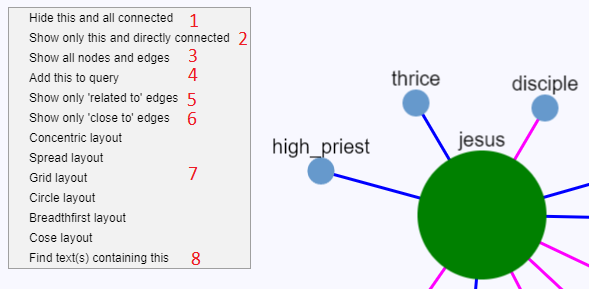
\includegraphics[scale=0.8]{fig/graph-interface}
    \caption{Overview of "dragn" result graph and options}
    \label{fig:graph-options}
\end{figure}
\begin{itemize}
    \item 1: Hides the selected node and all connected nodes.
    \item 2: Hides all but the selected node and all connected nodes.
    \item 3: Shows all previously hidden nodes.
    \item 4: Adds the token to the query.
    \item 5: Shows only the "related to" edges, the ones described in chapter \ref{sec:kbcompute}.
    \item 6: Shows only the "close to" edges, the ones described in chapter \ref{sec:kbcreate}.
    \item 7: Layout options for the nodes.
    \item 8: Adds the token to the context reader.
\end{itemize}
The context reader has been briefly mentioned in \ref{subsec:navbar}. It allows the user to scroll to paragraphs containing a certain word to get better understanding of either the relations it has with other words or to gain more understanding of the word itself by reading the paragraphs it appears in.


\subsection{Result graph}
\label{sec:resultgraph}
A result graph can be seen in figure \ref{fig:graph-options}.\\
The result graph is interactive and created with Cytoscape.js \cite{doi:10.1093/bioinformatics/btv557}, \cite{Cytoscapejs}. By default the ordering is random, but different automatic node alignments are available.\\
The following relations can be found in the result graph:
\begin{table}[H]
\centering
    \begin{tabular}{|l|l|}
    \hline
    colour & meaning\\
    \hline
    blue & close to, FMI-based \\
    red &related to, Cosine Similarity based on FMI scores \\
    magenta/pink & both close to and related to\\
    \hline
\end{tabular}
\caption{Explanation of edge colours}
\label{tab:relation_meaning}
\end{table}

\subsection{Result paragraphs and relations}
Each query produces not only the result graph, but a list of paragraphs relevant to the query with relations relevant to the query that appear in those paragraphs.\\
The paragraphs are scored based on their relevancy to the query as described in chapter \ref{sec:querystep}, with the highest scoring paragraph having a score of 1. For each paragraph the contained relations that are relevant to the query are shown in a sortable table, containing both the relations based on the FMI (see chapter \ref{sec:kbcreate}) as well as those over the cosine similarity (see \ref{sec:kbcompute}).\\
Additionally each paragraph in the result has buttons for "Previous" and "Next" paragraphs, respectively showing the paragraph preceding or following the paragraph for which the button was pressed in an overlay, which contains the same buttons. With this it is possible to get additional understanding of a certain paragraph by reading the paragraphs surrounding it.\\
Words in the result paragraphs can be added to the query directly by simply clicking them, thus allowing the user to explore possible links found in the paragraphs directly and easily.



\section{Summary of the architecture overview}
\textbf{dragn} consists of a pipeline of steps, where the output of the previous step forms the basis for the next step. They are:
\begin{itemize}
\item Splitting the texts into paragraphs and extracting Noun Phrases as described in \ref{sec:extract}
\item Calculating the modified PMI, the FMI, to establish connections between tokens in the texts, \ref{sec:kbcreate}
\item Calculating the Cosine Similarity based on the FMI of the tokens, as shown in \ref{sec:kbcompute}
\item Formatting the results into files to use for the queries, \ref{sec:indexstep}
\item Performing the queries based on the available data of the processed texts, as produced in the previous steps, was described in chapter \ref{sec:querystep}
\end{itemize}
The system was built upon the foundation of "Skimmr", the predecessor tool developed by Vit Novacek, who has written about it in \cite{novavcek2014skimmr}.\\
The code of the new system is up to current technical standards and a more intuitive user interface lets the user perform their tasks better and helps them understand the connections between tokens in their texts better.
Next follows an example use case utilising the new system's capabilities.